\chapter{Appendix A}

\section{Additional Apparatus Pictures} \label{sec:additional_apparatus}

\begin{figure}[htpb]
    \centering
    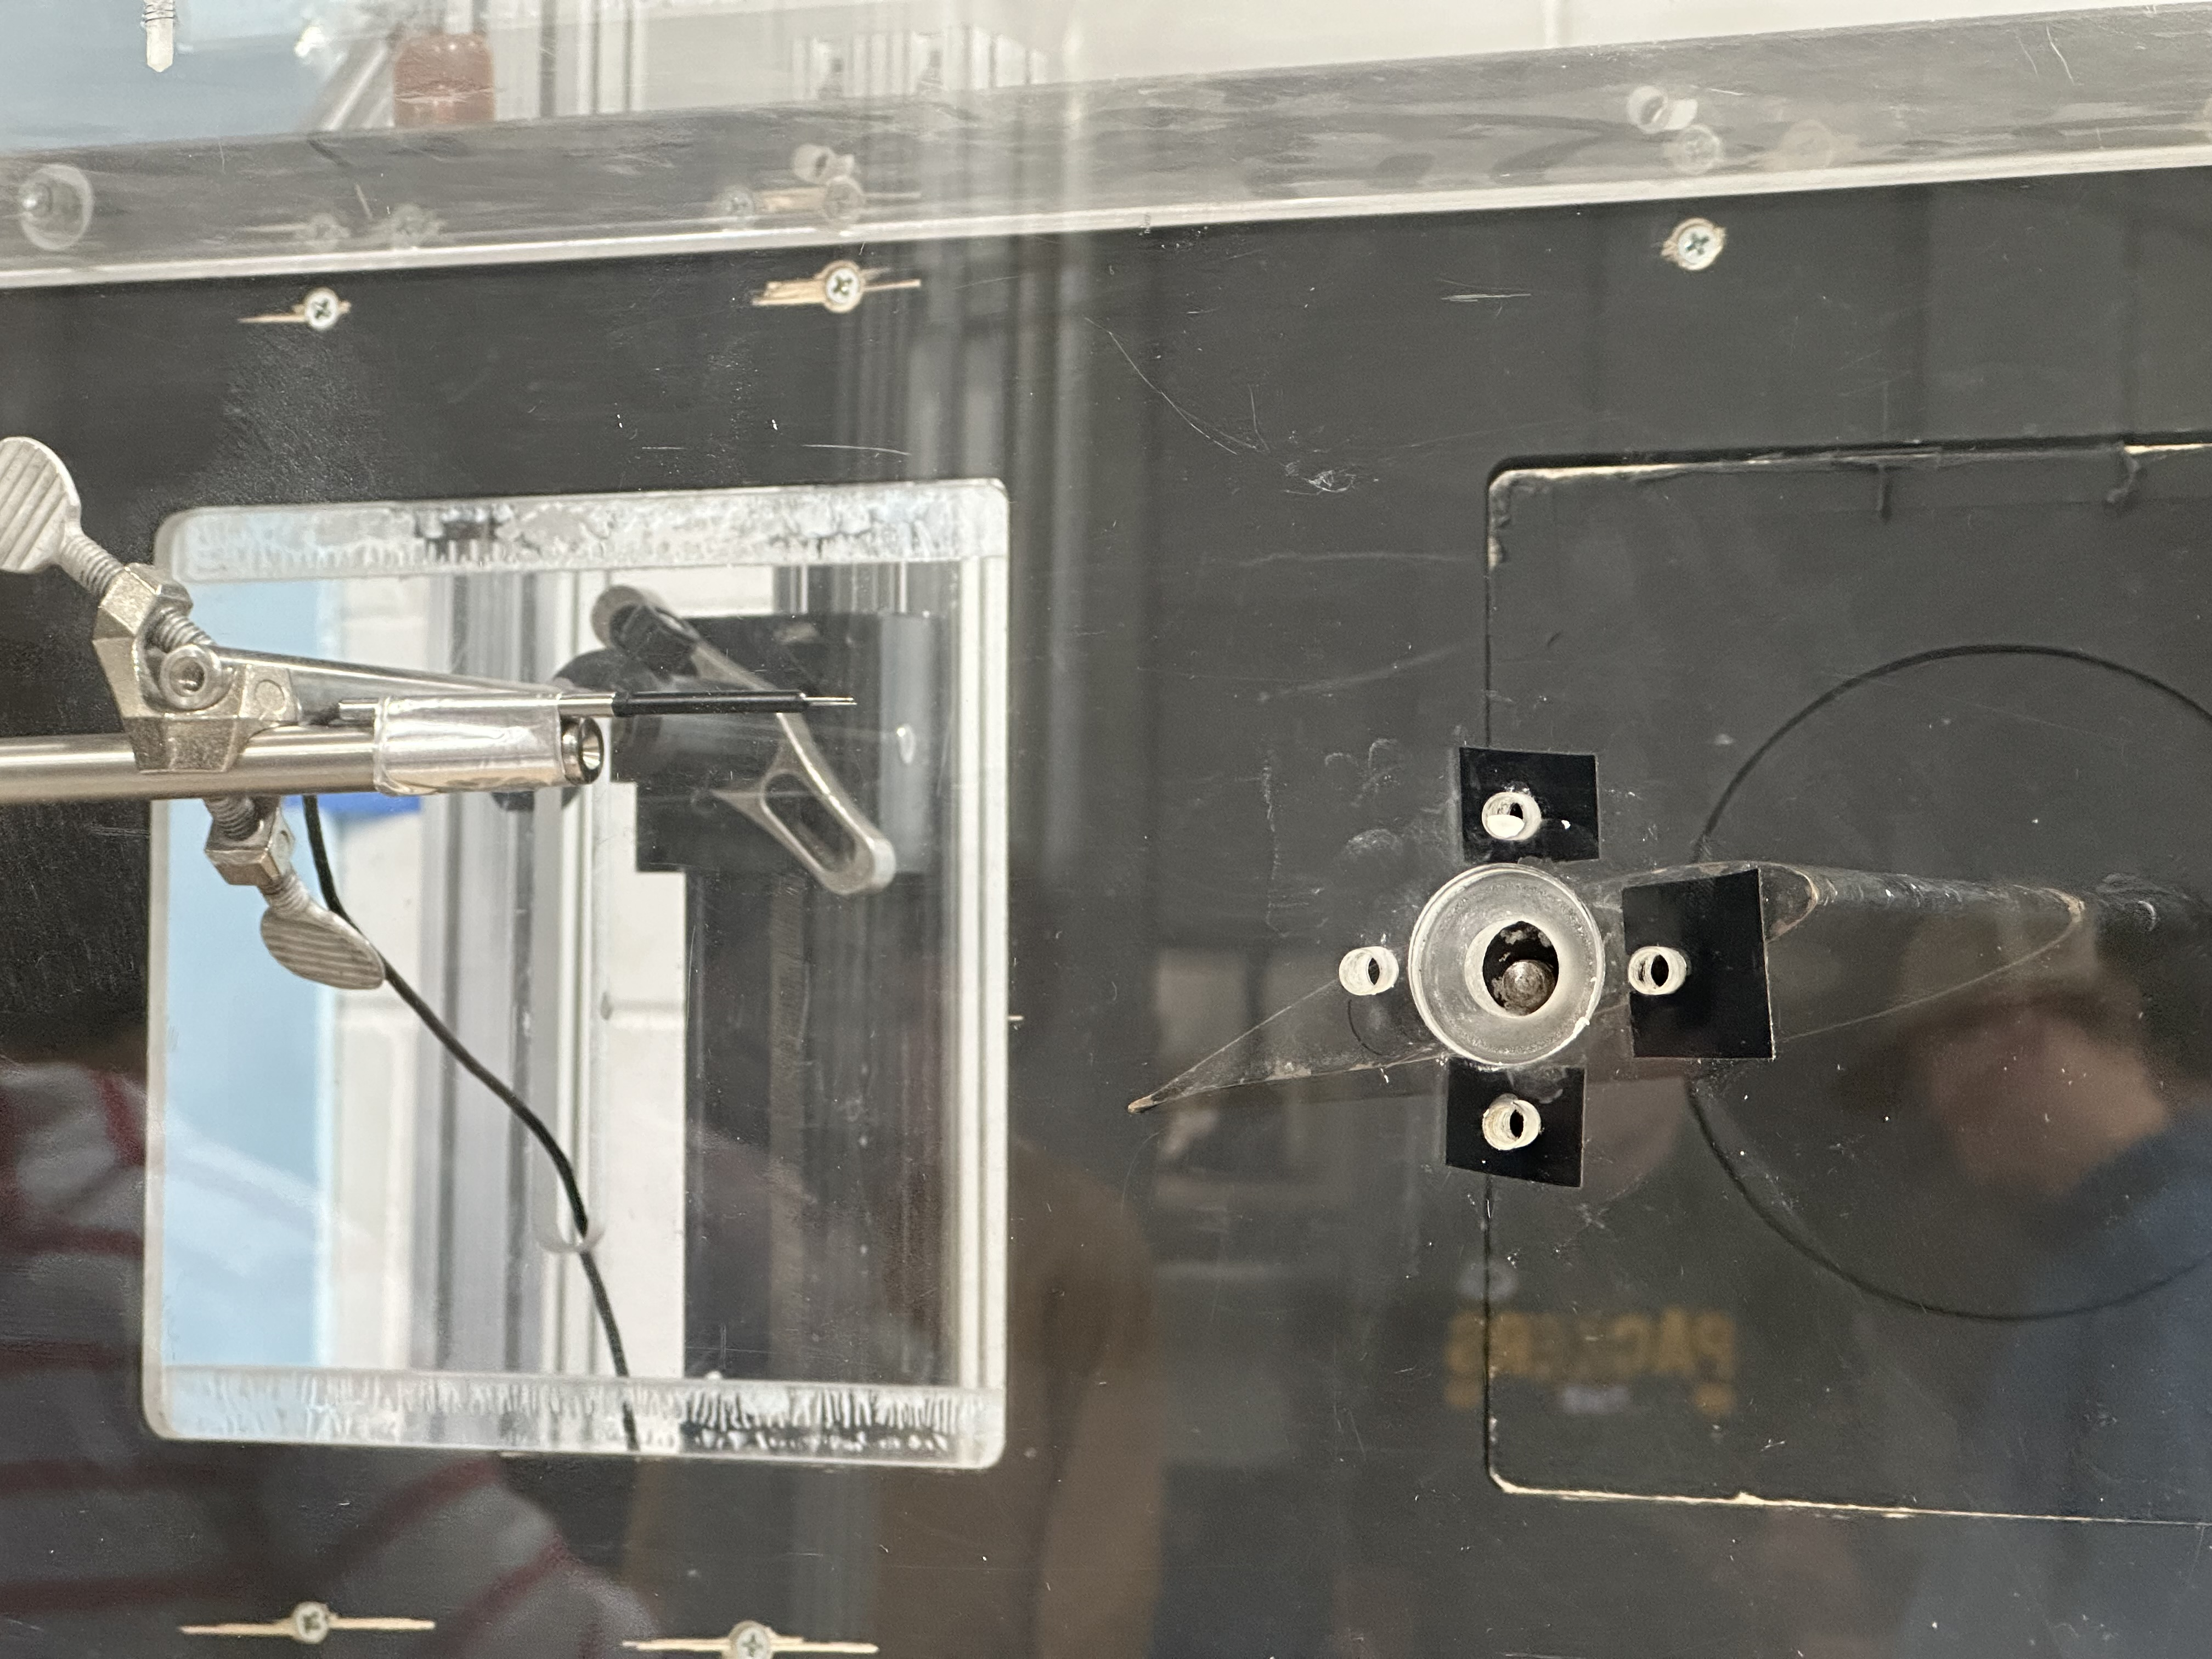
\includegraphics[width=0.75\linewidth]{Figures/IMG_3205.jpg}
    \caption[Hot Wire Anemometer behind the airfoil in the test section.]{Hot Wire Anemometer behind the airfoil in the test section.}
    \label{fig: HotWireAnemometerclose}
\end{figure}

\begin{figure}[htpb]
    \centering
    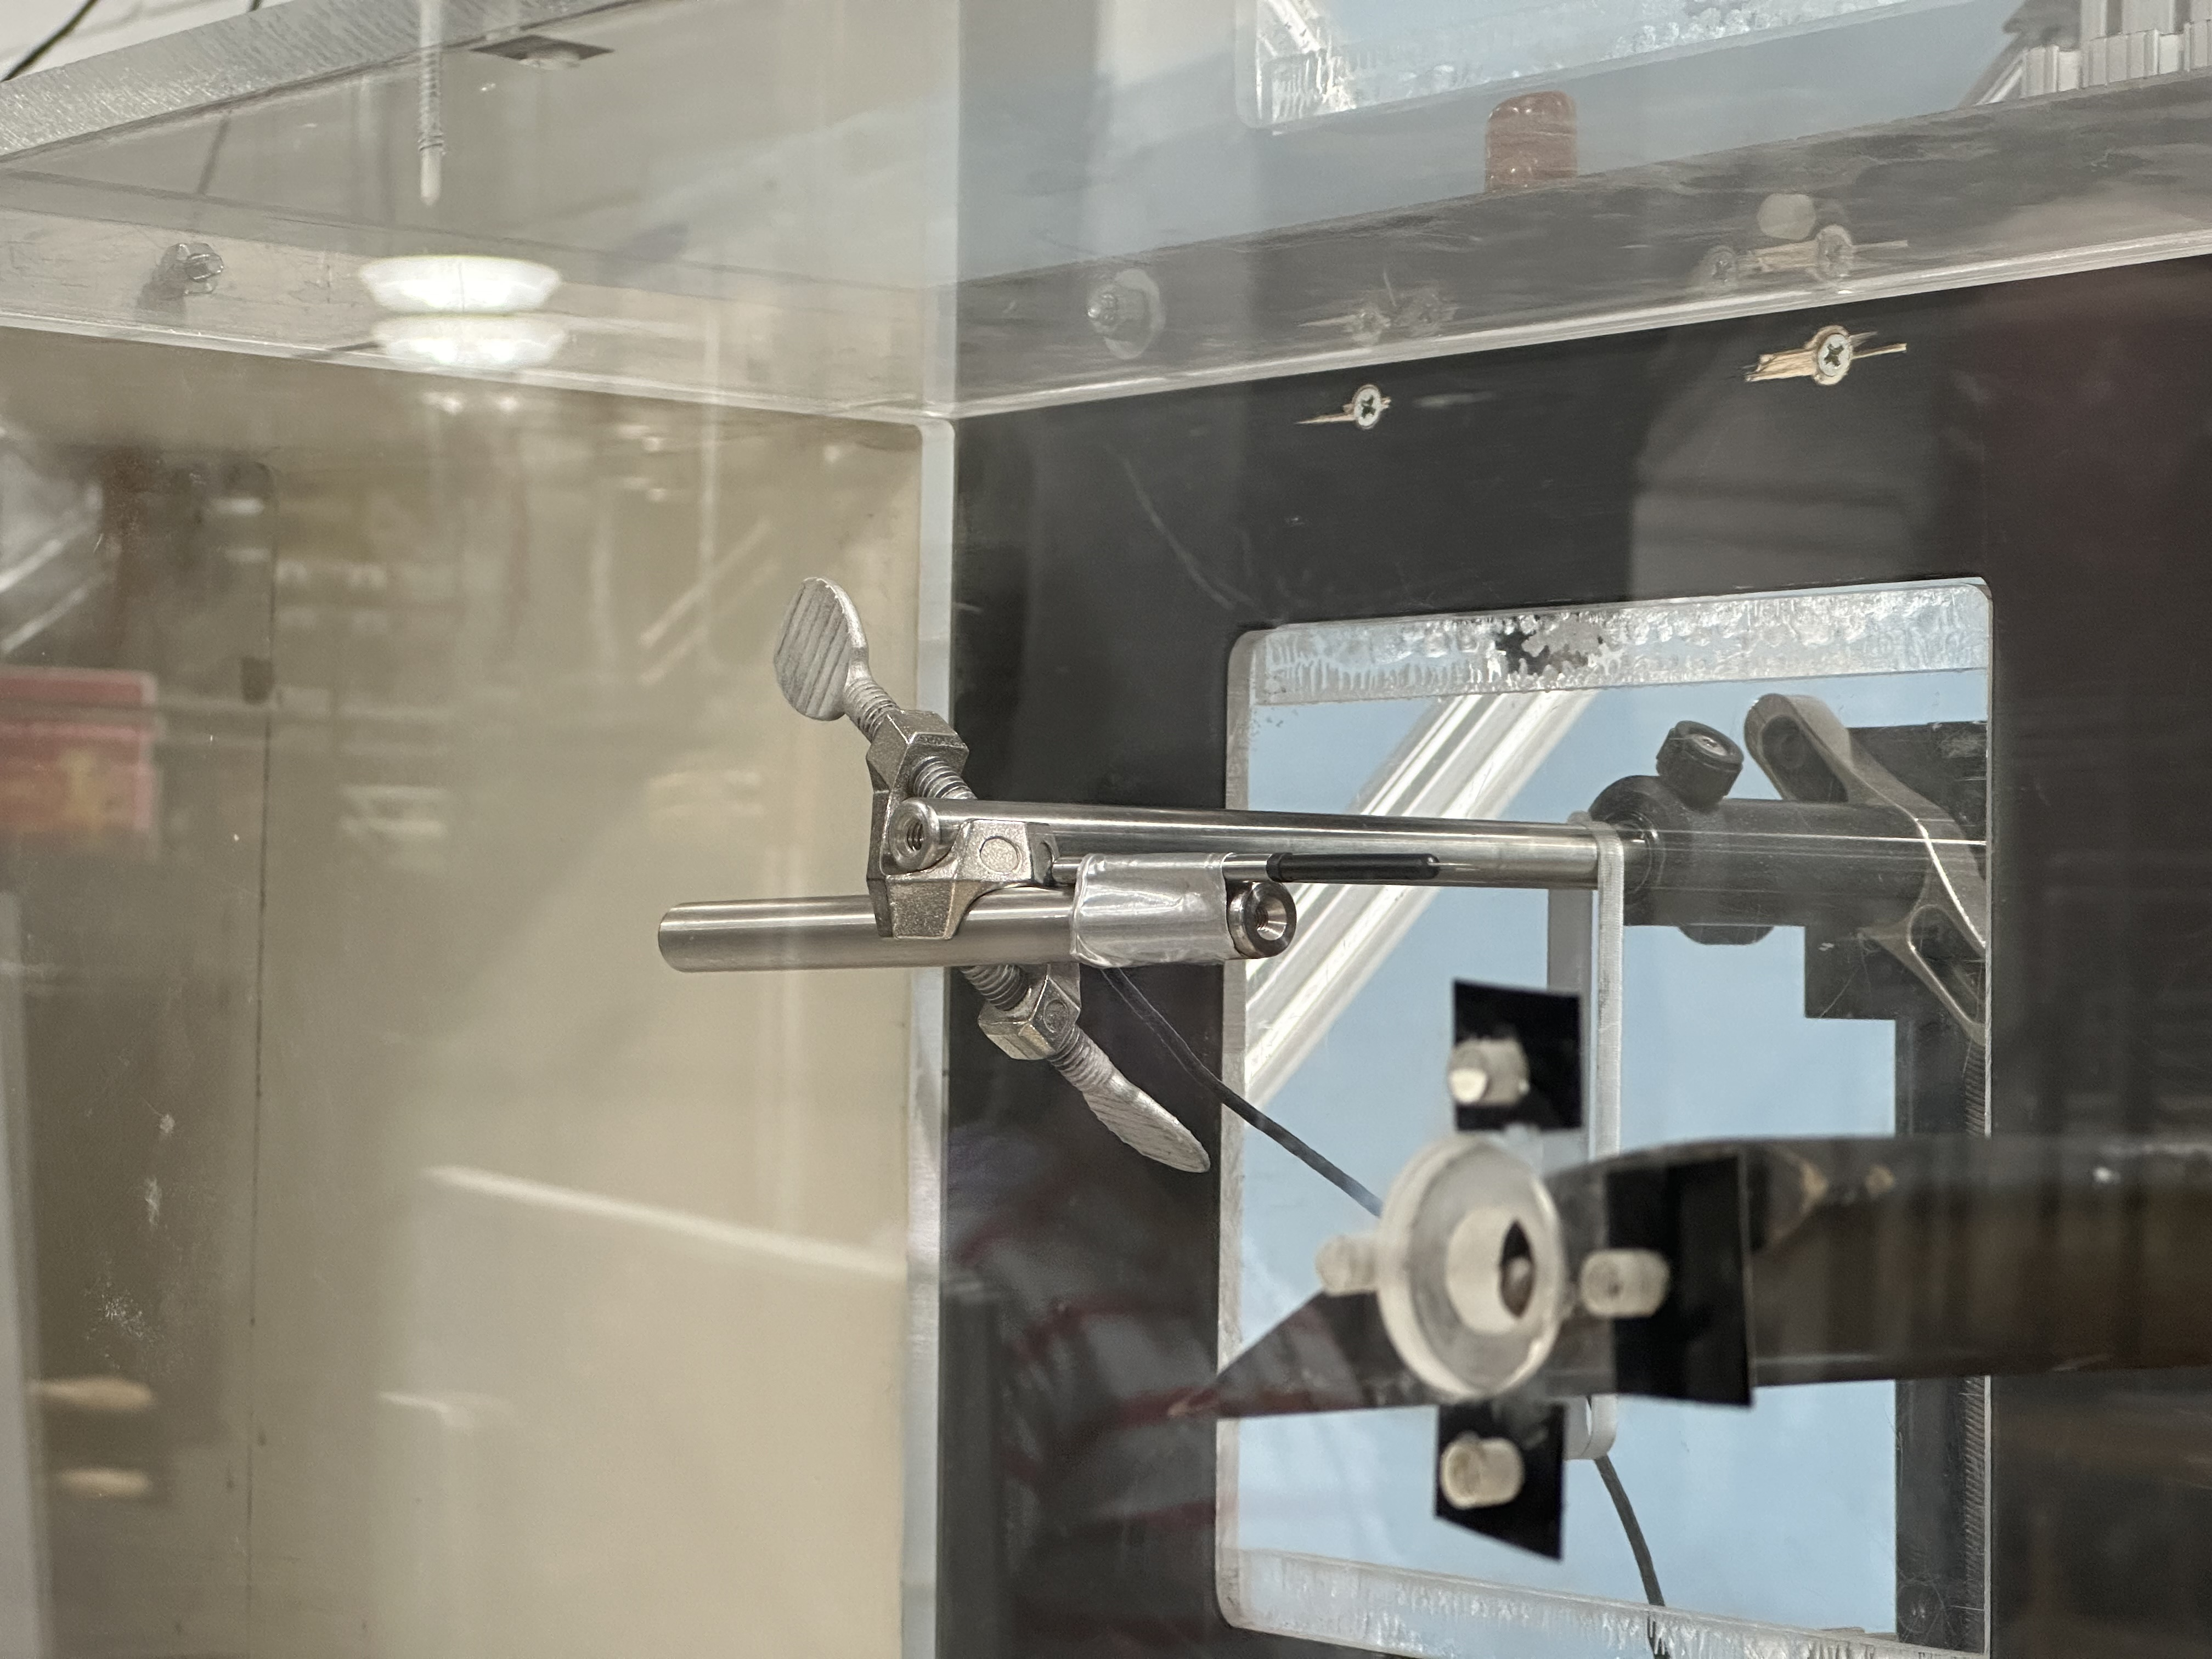
\includegraphics[width=0.75\linewidth]{Figures/IMG_3206.jpg}
    \caption[Hot Wire Anemometer behind the airfoil in the test section.]{ Wire Anemometer behind the airfoil in the test section.}
    \label{fig: HotWireAnemometerfront}
\end{figure}

\begin{figure}[htpb]
    \centering
    \includegraphics[width=0.75\linewidth]{Figures/IMG_3209.jpg}
    \caption[Adjustable knob to change the angle of attack of the airfoil.]{Adjustable knob to change the angle of attack of the airfoil.}
    \label{fig: SpeedControl}
\end{figure}

\newpage

\section{Additional Figures} \label{sec:additional_figures}

% template
% \begin{figure}[htpb]
%     \centering
%     \includesvg[width=0.75\linewidth]{Figures/Single-Sided Amplitude Spectrum at 4 AOA.svg}
%     \caption[A graph of the single-sided amplitude spectrum inside and outside the wake at a four degree angle of attack.]{The single-sided amplitude spectrum inside and outside the wake region at a \qty{4}{\degree} \acrshort{aoa}.}
%     \label{fig:Ydelta_vs_UUe_4AoA}
% \end{figure}

%\begin{figure}[htpb]
 %    \centering
 %    \includesvg[width=0.75\linewidth]{Figures/Single-Sided Amplitude Spectrum at 4 AOA.svg}
  %   \caption[A graph of the single-sided amplitude spectrum inside and outside the wake at a four degree angle of attack.]{The single-sided amplitude spectrum inside and outside the wake region at a \qty{4}{\degree} \acrshort{aoa}.}
   %  \label{fig:SSAS_at_4AoA}
%\end{figure}

\begin{figure}[htpb]
     \centering
     \includesvg[width=0.75\linewidth]{Figures/Single-Sided Amplitude Spectrum at 8 AOA.svg}
     \caption[A graph of the single-sided amplitude spectrum inside and outside the wake at a eight degree angle of attack.]{The single-sided amplitude spectrum inside and outside the wake region at a \qty{8}{\degree} \acrshort{aoa}.}
     \label{fig:SSAS_at_8AoA}
\end{figure}

\begin{figure}[htpb]
     \centering
     \includesvg[width=0.75\linewidth]{Figures/Single-Sided Amplitude Spectrum at 12 AOA.svg}
     \caption[A graph of the single-sided amplitude spectrum inside and outside the wake at a twelve degree angle of attack.]{The single-sided amplitude spectrum inside and outside the wake region at a \qty{12}{\degree} \acrshort{aoa}.}
     \label{fig:SSAS_at_12AoA}
\end{figure}

\begin{figure}[htpb]
     \centering
     \includesvg[width=0.75\linewidth]{Figures/Single-Sided Amplitude Spectrum at 16 AOA.svg}
     \caption[A graph of the single-sided amplitude spectrum inside and outside the wake at a sixteen degree angle of attack.]{The single-sided amplitude spectrum inside and outside the wake region at a \qty{16}{\degree} \acrshort{aoa}.}
     \label{fig:SSAS_at_16AoA}
\end{figure}

%\begin{figure}[htpb]
   %  \centering
   %  \includesvg[width=0.75\linewidth]{Figures/Ydelta vs. Turbulence Intensity at 4 AOA.svg}
  %   \caption[A graph of turbulence intensity vs position.]{Turbulence intensity at a \qty{4}{\degree} \acrshort{aoa}.}
   %  \label{fig:Ydelta_vs_TI_4AoA}
%\end{figure}

\begin{figure}[htpb]
     \centering
     \includesvg[width=0.75\linewidth]{Figures/Ydelta vs. Turbulence Intensity at 8 AOA.svg}
     \caption[A graph of turbulence intensity vs position.]{Turbulence intensity at a \qty{8}{\degree} \acrshort{aoa}.}
     \label{fig:Ydelta_vs_TI_8AoA}
\end{figure}

\begin{figure}[htpb]
     \centering
     \includesvg[width=0.75\linewidth]{Figures/Ydelta vs. Turbulence Intensity at 12 AOA.svg}
     \caption[A graph of turbulence intensity vs position.]{Turbulence intensity at a \qty{12}{\degree} \acrshort{aoa}.}
     \label{fig:Ydelta_vs_TI_12AoA}
\end{figure}

\begin{figure}[htpb]
     \centering
     \includesvg[width=0.75\linewidth]{Figures/Ydelta vs. Turbulence Intensity at 16 AOA.svg}
     \caption[A graph of turbulence intensity vs position.]{Turbulence intensity at a \qty{16}{\degree} \acrshort{aoa}.}
     \label{fig:Ydelta_vs_TI_16AoA}
\end{figure}

% \begin{figure}[htpb]
 %    \centering
 %    \includesvg[width=0.75\linewidth]{Figures/Ydelta vs. UUe at 4 AOA.svg}
  %   \caption[A graph of normalized velocity vs position.]{Velocity at a \qty{4}{\degree} \acrshort{aoa}.}
  %   \label{fig:Ydelta_vs_UUE_4AoA}
% \end{figure}

\begin{figure}[htpb]
     \centering
     \includesvg[width=0.75\linewidth]{Figures/Ydelta vs. UUe at 4 AOA.svg}
     \caption[A graph of normalized velocity vs position.]{Velocity at a \qty{8}{\degree} \acrshort{aoa}.}
     \label{fig:Ydelta_vs_UUE_8AoA}
\end{figure}

\begin{figure}[htpb]
     \centering
     \includesvg[width=0.75\linewidth]{Figures/Ydelta vs. UUe at 12 AOA.svg}
     \caption[A graph of normalized velocity vs position.]{Velocity at a \qty{12}{\degree} \acrshort{aoa}.}
     \label{fig:Ydelta_vs_UUE_12AoA}
\end{figure}

\begin{figure}[htpb]
     \centering
     \includesvg[width=0.75\linewidth]{Figures/Ydelta vs. UUe at 16 AOA.svg}
     \caption[A graph of normalized velocity vs position.]{Velocity at a \qty{16}{\degree} \acrshort{aoa}.}
     \label{fig:Ydelta_vs_UUE_16AoA}
\end{figure}